% !TEX TS-program = arara
% arara: xelatex: { synctex: on, options: [-halt-on-error] } 
% arara: biber
% % arara: texindy: { markup: xelatex }
% %% arara: makeglossaries
% % arara: xelatex: { synctex: on, options: [-interaction=batchmode, -halt-on-error] }
% % arara: xelatex: { synctex: on, options: [-interaction=batchmode, -halt-on-error]  }
% % arara: clean: { extensions: [ aux, log, out, run.xml, ptc, toc, mw, synctex.gz, ] }
% % arara: clean: { extensions: [ bbl, bcf, blg, ] }
% % arara: clean: { extensions: [ glg, glo, gls, ] }
% % arara: clean: { extensions: [ idx, ilg, ind, xdy, ] }
% % arara: clean: { extensions: [ plCode, plData, plMath, plExercise, plNote, plQuote, ] }
%-----------------------------------------------------------------
\documentclass[11pt]{PalisadesLakesBook}
% \geomHDTV
% \geomLandscape
\geomHalfDTV
\geomPortraitOneColumn
%-----------------------------------------------------------------

%\AsanaFonts % misssing \mathhyphen; less on page than Cormorant/Garamond
%\CormorantFonts % light, missing unicode greek
\EBGaramondFonts % fewest pages
%\ErewhonFonts
%\FiraFonts % tall lines, all sans, much less per page, missing \in?
%\GFSNeohellenicFonts 
%\KpFonts
%\LatinModernFonts
%\LegibleFonts
%\LibertinusFonts
%\NewComputerModernFonts
%\STIXTwoFonts
%\BonumFonts % most pages
%\PagellaFonts

%\ScholaFonts
%\TermesFonts
%\XITSFonts

%-----------------------------------------------------------------
\togglefalse{plMath}
\togglefalse{plCode}
\togglefalse{plData}
\togglefalse{plNote}
\togglefalse{plExercise}
\togglefalse{plQuote}
\togglefalse{printglossary}
\togglefalse{printindex}
%-----------------------------------------------------------------
\title{Notes on typography}
\author{John Alan McDonald 
(palisades dot lakes at gmail dot com)}
\date{draft of \today}
%-----------------------------------------------------------------
\begin{document}
\maketitle
\PalisadesLakesTableOfContents{7}
%-----------------------------------------------------------------
\def\sharedFolder{../../shared/}
%-----------------------------------------------------------------
\begin{plSection}{Introduction}

This is a collection of notes on font design,
typesetting (both for text and mathematics),
and possibly related layout problems. 
Partially notes on reading; 
partially my own work-in-progress analysis and implementation.
%-----------------------------------------------------------------
\begin{plSection}{Organizing thoughts}

\begin{itemize}

\item Better handwriting, rather than reproduce the best
traditional lead typesetting.

\item \emph{Question:} Compare evolution from handwriting to 
typesetting (including font development) for
math and 
汉字/\allowbreak 漢字/\allowbreak Hànzì/\allowbreak Kanji/\allowbreak Hanja/\allowbreak \mbox{Chữ Nôm}?\\
\citeAuthorYearTitle{MoteChu:1989:CalligraphyEABook}\\
\citeAuthorYearTitle{Kraus:1991:BrushesWithPower}
 
\item What could I (or somebody) do better
if I (they) were going to replace \TeX, \LaTeX, etc.


\end{itemize}
%-----------------------------------------------------------------
\end{plSection}%{Organizing thoughts}
%-----------------------------------------------------------------
\end{plSection}%{Introduction}
%-----------------------------------------------------------------
\begin{plSection}{Reading}
%-----------------------------------------------------------------
\begin{plSection}{Knuth}

\citeAuthorYearTitle{Coueignoux:1975:GenerationOfFonts}

\citeAuthorTitle{wiki:Metafont}

\citeAuthorYearTitle{Knuth:1979:MathTypography}

\citeAuthorYearTitle{Knuth:1982:MetafontConcept}

\citeAuthorYearTitle{Knuth:1989:TypesettingConcreteMath}

\citeAuthorYearTitle{Krantz:2001:MathTypography}

\citeAuthorYearTitle{Beebe:2005:DesignTexMetafont}

\citeAuthorYearTitle{Crossland:2008:WhyMetafontDidntCatchOn}

\citeAuthorYearTitle{BeetonPalais:2016:CMT}

\citeAuthorYearTitle{Smith:2017:MathTypography}.

\citeAuthorYearTitle{McCarthy:2020:StanfordDigitalTypography}

\end{plSection}%{Knuth}
%-----------------------------------------------------------------
\begin{plSection}{Unicode Math}\label{sec:UnicodeMath}

\citeAuthorYearTitle{BeetonEtAl:2014:UnicodeMath}

\end{plSection}%{OpenType}
%-----------------------------------------------------------------
\begin{plSection}{OpenType}\label{sec:OpenType}


\end{plSection}%{OpenType}
%-----------------------------------------------------------------
\begin{plSection}{Microsoft}

\citeAuthorYearTitle{MillsHudsonLawrenceSargent:2007:MSMathTypesetting}

%-----------------------------------------------------------------
\begin{plSection}{ClearType}\label{sec:ClearType}
\citeAuthorTitle{wiki:ClearType}
\end{plSection}%{ClearType}
%-----------------------------------------------------------------
\end{plSection}%{Microsoft}
%-----------------------------------------------------------------
\begin{plSection}{Math style guides}
%-----------------------------------------------------------------
\begin{plSection}{American Mathematical Society}

\citeAuthorYearTitle{Swanson:1999:MathIntoType}

\citeAuthorYearTitle{LetourneauSharp:2017:AMSStyleGuide}

\end{plSection}%{American Mathematical Society}
%-----------------------------------------------------------------
\begin{plSection}{London Mathematical Society}

\citeAuthorYearTitle{RoddTornqkvist:2009:LMSStyleGuide}

Seems aimed at traditional kind of typesetting:
paper(?) copy marked in pencil(?)  
passed on to typesetter for formatting.

Interesting typo? on p $21$: ``$\theta$ vs $\mathscr{V}$''

Useful list of ``mathematical statement'' types.

Slanted fonts for emphasis; no italic in text;
math variables italic/roman by author's choice.

Latex commands used to communicate with typesetter.


\end{plSection}%{London mathematical Society}
%-----------------------------------------------------------------
\begin{plSection}{Oxford University Press}

\citeAuthorYearTitle{ChaundyBarrettBatey:1954:PrintingMathematics}

\end{plSection}%{Oxford University Press}
%-----------------------------------------------------------------
\end{plSection}%{Math style guides}
%-----------------------------------------------------------------
\begin{plSection}{Noordzij}

\citeAuthorTitle{Devroye:2014:Noordzij}

\citeAuthorTitle{Middendorp:2019:Noordzij}

\end{plSection}%{Noordzij}
%-----------------------------------------------------------------
\begin{plSection}{Rhatigan}
%-----------------------------------------------------------------
\begin{plSection}{\citeAuthorYearTitle{Rhatigan:2007:Monotype4Line}}
\label{sec:FourLine}

A 38 page essay reviewing the Monotype (UK)
4-line system for mathematics typesetting.
The essay doesn't put much attention on the chronology
(probably covered well in the references),
but it appears that the development
began some time shortly after the end of WWII,
with the first installed system in June of 1958.
This appears to be roughly contemporaneous with
the development of the Monotype Filmsetter,
which (I'm guessing) made the hot lead type machines 
obsolete.~\cite{Eye:2012:MonotypeTimeline}

\emph{Question:} What, if anything, can we learn from the
4-line system that is relevant to digital typesetting
of mathematics?

\emph{Question:} To what extent did the limitations of
hot lead typesetting, of any kind, 
fail to reproduce math notation as practiced by mathematicians?
To what extent are these (now unnecessary) restrictions
carried over (perhaps unconsciously) into digital typesetting,
and webpage layout?

\begin{plQuote}
{\citeAuthorYearTitle[p.~11]{Rhatigan:2007:Monotype4Line}}
{PostwarMonotype}
As it resumed production in the wake of the war,
Monotype found itself struggling to meet its customers'
demands for parts and equipment. 
In this climate of an uncertain return to economic stability,
it makes sense that the company would choose to develop
technology such as the 4-line system that adapted to its existing
equipment and working methods, 
rather than solutions that would make unrealistic demands
on the company's ability to devise and manufacture 
new kinds of equipment altogether. 
\end{plQuote}

Idea seems to be 4 half-lines, with extra 2pt spaces between the 
upper and lower pairs.
Half-lines wide (high) enough for sub/super script chars;
2 half-lines (roughly?) equivalent to normal char height, 
normal line of text.
The extra 2pt space is to allow for clean horizontal rules in
fractions.
Examples (fig 8, 9) show integrals $\int$ 
taking advantage of 
available double line height, but not sums $\sum$,
and the sum readability suffers.

Figures 9 and 10 compare a traditional setting with 4-line result,
and, although neither looks good to me,
the 4-line is a little better,
though that's primarily because the greek letters 
in the traditional setting are too small,
as mentioned in the captions.
In figure 10, however, although the kerning of 
$L^2$ is a bit better, other spacing is screwed up:
\begin{itemize}
\item $\sin^2 \,\omega$ rather than $\sin^{2}\!\omega$ or, even better, 
 $\textrm{sin}^{2}\!\left(\omega\right)$
\item $v_{\,1}\;,\;v_{2}$ rather than $v_{1},v_{2}$
\item $\sum\,'$ rather than $\sum^{'}$
\end{itemize}

Developed together with Times 4-line Mathematics Series 569 font
derived from Times New Roman Series 327. 

\begin{plQuote}{\citeAuthorYearTitle[p.~21]{Rhatigan:2007:Monotype4Line}}
{}
Planning the correct keying sequence is a critical part of the
training for a keyboard operator setting maths.
Rather [than] reading through manuscript text 
in a linear fashion,
the operator needs to examine each equation in a manuscript,
determine how much of it can be set mechanically,
and then how the characters and symbols within that equation
should be positioned within the 4 available lines. 
\textit{(See figure 13.)}
For any characters that cannot be set in line with the others
(characters larger than 12 points, for example,
or additional symbols that could not be fit into the matrix case),
spaces of equal width (removed by the compositor later)
are needed to hold their position for justification.
\end{plQuote}

\begin{plQuote}{\citeAuthorYearTitle[p.~25]{Rhatigan:2007:Monotype4Line}}
{}
\ldots increased the speed of maths composition 
by an average of 26 percent.
\end{plQuote}

\begin{plQuote}{\citeAuthorYearTitle[p.~25]{Rhatigan:2007:Monotype4Line}}
{}
Series 569 and the principles of the 4-line layout 
were even adapted for Monophoto---Monotype's 
filmsetting technology---and their relevance carried on 
until the digital era demand other solutions 
for setting mathematics.
\end{plQuote}

\emph{Conclusions:}
Seems fundamentally limited. 
No doubt a reasonable economic compromise given the technology of
the time, but not a model for high-resolution digital typesetting.

For additional history, see
\citeAuthorYearTitle{Smith:2017:MathTypography}.

\emph{Note:} \TeX was invented, at least in part, 
to reproduce the perceived superior quality 
of 4-line Monotype setting
in the first edition of Knuth, The Art of Computer Programming
(see \citeAuthorYearTitle{BeetonPalais:2016:CMT}).

\end{plSection}%{The Monotype 4-line system}
%-----------------------------------------------------------------
\begin{plSection}{Gina}

\begin{plSection}{\citeAuthorYearTitle{Rhatigan:2007:GinaPractice}}

A 40 page essay on the experience of developing the type family
Gina.

\begin{plQuote}{\citeAuthorYearTitle[p.~1]{Rhatigan:2007:GinaPractice}}{}
This document is more an analysis of that process of discovery
[for designing a typeface]
than a guide to designing type.
The missteps and the inefficiencies discussed, though, 
point the way to more sound methods for 
Gina's own future development as well as that of other typefaces.
\end{plQuote}

Section 2.1: Gina intended as a serif typeface 
``matching math to the text''.

(\emph{Comment:} Not a desirable goal for me, depending
on what ``matching'' means.
Important to easily distinguish math notation from normal text,
especially when mixed. 
Analogy to 漢字\allowbreak ひらがな\allowbreak カタカナ\allowbreak romaji
(kanji hirgana katakana romaji) pre-parsed Japanese text?)


\begin{plQuote}{\citeAuthorYearTitle[p.~3]{Rhatigan:2007:GinaPractice}}{}
Gina was originally conceived as a serif typeface family
for textbooks and other technical publications that may include
equations, chemical formulas, tables, and other combinations of
text, numerals, and symbols.
Material like this requires type that will facilitate long dense
passages of text, but it must also feature glyphs with enough
individual clarity that they can be recognized outside of typical
word shapes, such as in mathematical or chemical formulae.
\end{plQuote}

\emph{Comment:} 
Compare to \citeAuthorYearTitle{Braille:2021:AtkinsonHyperlegible},
\citeAuthorYearTitle{DobieScottScott:2021:AtkinsonHyperlegible}.

References \citeAuthorYearTitle{Bouche:2003:DiversityMathFonts}.

Figure 4 compares Gina to more conventional set of fonts:
\begin{itemize}
  \item Gina digits too small in $2i$ and $1.0\,g$, 
  should either descend below baseline ot rise above x-height.
  \item Gina $3/4$ is too small.
  \item Conventional setting seems to use slanted rather 
  than italic capitals, which I find easier to read, less cramped.
  \item Gina's rounder italic $\mathit{a}$ is better; 
  probably upright sans would be better still.
  \item Gina seems to get heavier as Adobe Reader zooms in?
  Conventional setting feels like the same weight regardless. 
\end{itemize}

Design process began, in class, with pencil sketches on paper,
starting from Morris Fuller Benton's New Century 
Schoolbook~[p.~7].
Pencil sketches scanned and traced~[p.~8, fig.~7] 
in FontLab Studio 5.0.2~\cite{FontLab:2021}.

\begin{plQuote}{\citeAuthorYearTitle[p.~9]{Rhatigan:2007:GinaPractice}}{}
Concentrating on the outlines often resulted in clear details
but distorted characters overall.
Calligraphy exercises, attempted without much experience 
using a broad nib pen, resulted in letters too crude
to be helpful. Drawing directly in FontLab was just as awkward
at this beginning stage.

A technique of jotting down some key positions on paper
before connecting parts of the contours---building up from gestural
lines and basic proportions to overall shapes 
and then on to finer elements, 
refining the good lines and slowly eliminating the bad ones---was
somewhat more helpful.
Rather than collage of connected details,
these drawings produced an overall \emph{sense of mass} 
and \emph{relationships between parts.}
Made with larger motions fo the arm and the hand,
the straight lines had more \emph{tension}
and the curves had more \emph{swing} 
the the slower, more deliberate contour drawings.
[\emph{Emphasis} added.]
\end{plQuote}

\emph{Question:}
Can we quantify \emph{mass} and \emph{relationships},
and optimize \emph{tension} and \emph{swing}?

Section 3.3: experience with non-Latin (Indic and Greek) 
scripts helpful~[figs.~8,~9]. Broad nibbed pen for Devanagari
and unspecified ``rounder tool'' for greek.

\begin{plQuote}{\citeAuthorYearTitle[p.~11]{Rhatigan:2007:GinaPractice}}{}
The insights from these two workshops into the relationship
of action and form led to some different sketching
techniques---particularly the use of pen and ink 
to experiment with discrete shapes as well as entire 
letters---that fed into Gina's eventual design.
\textit{(See figures 10 and 11.)}
They also led to a means of distinguishing similar forms
in the roman, italic, and Greek glyphs:
using the writing tradition to guide the overall look
of each set of shapes in a slightly different direction.
\end{plQuote}

Figure 10 shows ideal singularities the result from two pencils
tied together to simulate and edged pen: the two curves cross over
as the 'pen' changes direction --- invisible 
with an actual edged pen because the ink path never goes 
completely to zero width.

\emph{TODO:} Work this out in a little more detail. 
Cross-over happens the direction of motion passes thru parallel 
to the pen edge.

\emph{TODO:} 
Compare this to \citeAuthorYearTitle{Noordzij:2006:TheStroke}.

\emph{TODO:} the below in not quite right.
Want something that can be filled to simulate ink.
That requires connecting the left and right curves
at extrema, in some sense.

\emph{TODO:} must be some way to define the central path just once? 
See CTAN calligraphy?
Or \url{https://tex.stackexchange.com/questions/19715/programming-in-tikz/19720#19720}


\begin{plDiagram}{Stroking with an edged pen}{}
\center
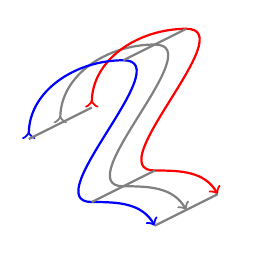
\begin{tikzpicture}
% \path[>->,thick,gray,draw,save path=\PenPath] (0mm,0mm) 
% to [out=90,in=180] (12mm,10mm)
% to [out=0,in=180] (8mm,-8mm) 
% to [out=0,in=120] (16mm,-11mm) ;
\path[>->,thick,gray,draw] (0mm,0mm) 
to [out=90,in=180] (12mm,10mm)
to [out=0,in=180] (8mm,-8mm) 
to [out=0,in=120] (16mm,-11mm) ;
\path[>->,thick,red,xshift=4mm,yshift=2mm,draw]
 (0mm,0mm) 
to [out=90,in=180] (12mm,10mm)
to [out=0,in=180] (8mm,-8mm) 
to [out=0,in=120] (16mm,-11mm) ;
\path[>->,thick,blue,xshift=-4mm,yshift=-2mm,draw] 
(0mm,0mm) 
to [out=90,in=180] (12mm,10mm)
to [out=0,in=180] (8mm,-8mm) 
to [out=0,in=120] (16mm,-11mm) ;
% pen edge sampled at control points
\path[thick,gray,draw] 
(-4mm,-2mm) to (0mm,0mm) to (4mm,2mm) ; 
\path[thick,gray,xshift=12mm,yshift=10mm,draw] 
(-4mm,-2mm) to (0mm,0mm) to (4mm,2mm) ; 
\path[thick,gray,xshift=8mm,yshift=-8mm,draw] 
(-4mm,-2mm) to (0mm,0mm) to (4mm,2mm) ; 
\path[thick,gray,xshift=16mm,yshift=-11mm,draw] 
(-4mm,-2mm) to (0mm,0mm) to (4mm,2mm) ; 
\end{tikzpicture}
\end{plDiagram}

\begin{plQuote}{\citeAuthorYearTitle[fig.~11]{Rhatigan:2007:GinaPractice}}{}
\ldots a closer look at more types 
by Dwiggins made it clear he was manipulating details to provide 
an even stronger sense of the pen stroke in small point sizes.
\end{plQuote}

Figure 17 shows a comparison of varying extender lengths
generated by FontLab, using two 'master' fonts generated by hand,
with one interpolation and two extrapolations.

\begin{plQuote}{\citeAuthorYearTitle[p.~21]{Rhatigan:2007:GinaPractice}}{}
The italic and Greek glyphs took cues from a tradition of
written forms just as Gina's roman did.
Although none of the styles would slavishly follow calligraphic 
shapes,
using these three distinct writing styles as a point of departure
for the design provided a means to distinguish the forms from one
another in text.
\end{plQuote}

Section 5: experience with roman made it possible
to draw italic and greek directly in FontLab.

Section 5.1: experiments with italic slope, by slanting roman.

Fig. 23: some greek pangrams~\cite{wiki:Pangram} 
to use in font testing.

Section 5.3: designing figures to match (roman? italic?)
more difficult than expected.

Fig 25: blocks of figures and symbols used to even out apparent
weight, to merge visually into other text---but that's probably
the wrong goal: certainly math symbols shouldn't disappear into
normal text, and maybe not numbers either.
Also, tested operators are much too small.

Fig.27: spacing test, unclear if the test was done at normal size
or at thumbnail size (thumbnail test would be wrong). Also. seems
like goal is even texture for mixture of math, greek, italic, 
roman; not likely the right goal.

Section 6: extended character set required 
``more systematic handling'' (automation?).
Not clear if he succeeded.
``{\ldots} most difficult aspect{\ldots}was constructing test
documents in Adobe InDesign{\ldots}''. 

(Why Adobe InDesign? 
Would {\LaTeX} help?
Software to find suitable, real examples of extended char set use 
in web pages and documents, pdf or something else?) 

(Reviewing lots of docs by eye seems difficult.
Might help to have a fixed test set plus continued sampling
of new docs.
Any possibility of partial automation, eg, variation in blurred
image, local 2d spectra.
Experimenting with image transforms that expose layout issues 
to the eye might be a way to find objective functions that
could be used for automated optimization of glyph design
and page layout.) 

Section 7: Future development. Gina unfinished, esp italic,
and math barely started.

\begin{plQuote}{\citeAuthorYearTitle[p.~31]{Rhatigan:2007:GinaPractice}}{}
This version of Gina was optimised for common desktop publishing
software (primarily so testing could be restricted to a 
manageable set of technical issues). 
In reality those are not the tools commonly used to typeset 
mathematics, and in the end Gina will probably need to be
re\"{e}ngineered for a different production environment.
\end{plQuote}
 
\begin{plQuote}{\citeAuthorYearTitle[p.~33]{Rhatigan:2007:GinaPractice}}{}
Many repetitive tasks such as repositioning components or
adjusting the stem height of new optical sizes are instructional 
the first few times,
but better handled by automation 
once the principles are understood.

{\ldots}
Learning to perceive and manipulate subtle variations in shape,
in weight, and in proportion was the most difficult part 
of this past year.
{\ldots} Learning how to discern---and hopefully enhance---the
relationships within a set of shapes became
an entirely new way to understand not only typefaces,
but also typography in a broader sense.
\end{plQuote}

\end{plSection}%{\citeAuthorYearTitle{Rhatigan:2007:GinaPractice}}
%-----------------------------------------------------------------
\begin{plSection}{\citeAuthorYearTitle{Rhatigan:2007:GinaSpecimen}}

Tabular oldstyle figures (digits) are nice and, I think,
relatively unusual.

(\emph{Unrelated Question:} 
Any font with quasi-oldstyle digits that alternate 
ascending above x-height and dropping below baseline?
Eg, 0 rising, 1 with a descender of some kind, 2 rising, 3 with
a descender (usual for oldstyle), 4 ascending (usual is descending).
The remaining 6--9 alternate ascending/descending in most
oldstyle digit renderings.
Don't know if this would actually look good.
Might be a project for learning FontForge?)

Mathematics examples are too limited to judge, 
but operators ($\int$, $\prod$) look too small. 
(How was the math in the specimen doc typeset?)

\end{plSection}%{\citeAuthorYearTitle{Rhatigan:2007:GinaSpecimen}}
%-----------------------------------------------------------------
\end{plSection}%{Gina}
%-----------------------------------------------------------------
\begin{plSection}{\citeAuthorYearTitle{Rhatigan:2007:MathTypefaces}}

\citeAuthorYearTitle{Lawrence:2003:MathsTypography}

\begin{plQuote}{\citeAuthorYearTitle[Introduction]{Rhatigan:2007:MathTypefaces}}{}
This dissertation will examine the design and function of
alphabetic characters of three typefaces created specifically for
mathematics---Times 4-line Mathematics Series 569,
\textsc{ams} Euler, and Cambria Math.

{\ldots}Each typeface represents a distinct period of technical
development, each in some sense reacting to the typefaces 
and technologies preceding it.

Times 4-line Mathematics Series 569 was created by the Monotype
Corporation in the United Kingdom for use with its hot-metal
composition equipment [introduced in 1957]{\ldots}.

\textsc{ams} Euler was designed by typographer and
calligrapher Hermann Zapf in collaboration with Donald E. Knuth
[circa 1979]{\ldots}.

Cambria Math was designed by Jelle Bosma [circa 2004--2007]
to take advantage of two major technologies from Microsoft: 
one a new way to improve the appearance of text 
displayed on screens, 
the other a sophisticated new method 
of creating and typesetting equations.
\end{plQuote}

\begin{plQuote}{\citeAuthorYearTitle[1.1 Typeface requirements, p.~5]{Rhatigan:2007:MathTypefaces}}{}
Mathematics is a field of study that employs its own vocabulary 
and conventions, and in many ways it has a language 
and writing system of its own. 
Although its notation uses many familiar characters, 
it uses them as symbols rather than words. 
However, maths is set alongside the words that convey its meaning, 
and publishing maths requires the ability to mix the symbolic 
and the verbal languages with one another.

Setting complex mathematics requires the use of a wide array 
of characters that must work in harmony. 
Numbers are mixed with alphabetic characters 
of Latin and Greek origin in a variety of styles — 
italic, bold, fraktur, serif and serif forms — 
each with a specific semantic function. 
All these characters are then mixed 
with mathematical operators and other symbols 
that often conflict with the scale or texture 
of the other characters. 
Setting maths, then, requires access to a vast set 
of unique characters, preferably ones 
that have been designed to work with one another. 
(See figure 1.)
\end{plQuote}

Problems:

This misses the connection to handwriting---on black/white boards
for dialog/teaching/collaboration, on paper for calculation, 
that is, symbolic computation.
The 'normal' text in typeset math
is, to some extent, a substitute for speech in the first case,
and something akin to comments in code in the second.

Another problem is ``specific semantic function'': 
there is no standard for the natural language that is 
math notation; 
it varies to some degree from individual to individual,
with dialects that are mutually unintelligible 
between different subfields.

Yet another issue is the apparent presumption of a clear division
between alphabetic symbols and operators, and, perhaps worse,
the assumption that there is a fixed, finite set of such glyphs.

Yet another: dialog math often includes pictures, diagrams 
(not in this case category theory diagrams), etc.,
that are mixed with math expressions.

\emph{Maybe important:} 
Writing systems are constrained by the nature of the writing
instrument and the writing surface.
For regular text, we have already seen an evolution away from
handwriting, given keyboard as writing instrument
and high resolution screen as surface.
In principle, this makes an entirely new math notation possible,
but not feasible unless keyboard/ mouse input enables
fluid dialog. 

Need for single character legibility, as opposed to word-shape
readability:
``mathematics'' vs ``mαthemαtics'' doesn't matter (maybe)
but ``x = a + 4'' vs ``χ = α + A'' are completely different.

%-----------------------------------------------------------------
\begin{plSection}{\citeAuthorYearTitle[2.1 Times 4-line Mathematics Series 569]{Rhatigan:2007:MathTypefaces}}

The 4-line hot lead system intended as cost cutting, 
not ideal solution.
(But was the inspiration for metafont and tex (reference?)).
Carried over into phototypesetting, 
even though there might have been better approaches there?

Discussion of 4-line system pretty much the same as in 
\cref{sec:FourLine}.

Brief outline of development of Times New Roman font,
released in 1931,
from Robert Granjon's Gros Cicero by way of Monotype Plantin.
Intended for newspaper printing,
``Times Roman achieved its popularity chiefly in general printing, 
not in newspaper work'' 
(\citeAuthorYearTitle{Tracy:1986:LettersOfCredit},
quoted in \cite{wiki:TimesNewRoman}),
The general popularity was due to compactness,
but few newspapers other than The Times
(of London) had the necessary high quality printing.

The Times 4-line Mathematics Series 569 
replaced Monotype's recommended use of Modern Series 327 
(says Series 7 in some places?) for math.
Took glyphs from various fonts, adjusted for the 4-line system.
Italic $16^{\circ}$ slant in 327 reduced to $12^{\circ}$ in 569.

Total matrices (glyph molds) initially about 750, 
up to 8000 by 1971. 
Rhatigan (or maybe Monotype) claim 11000 characters,
counting the same matrix used for super- and sub-scripts
as distinct.

\emph{Question:} would we ever want distinct glyphs 
for sub-and super-scripts?

Currently ``electronic'' version of 569 offered as font
``Math \& Technical 17''.

At this point, no evaluation of the font or 4-line typesetting.

\end{plSection}%{\citeAuthorYearTitle[2.1 Times 4-line Mathematics Series 569]{Rhatigan:2007:MathTypefaces}}{}
%-----------------------------------------------------------------
\begin{plSection}{\citeAuthorYearTitle[2.2 \textsc{ams} Euler]{Rhatigan:2007:MathTypefaces}}

Knuth and Zapf: 
``design experiment as much as a technical experiment''
(not sure what that means).

Knuth: METAFONT and {\TeX}

TeX: a ``command language''. Brief discussion of boxes and glue.
``{\ldots}each document contains complete information 
about how it should look''~[p~19]. 
(Not true, in any practical sense,
since the results are unstable w.r.t. small changes in content,
and therefore unpredictable. Also, practical use means depending
on 100s, in not 1000s, of libraries (aka packages) 
with rapidly propagating dependencies, 
with updates every month or so.)

Metafont: brief, uncritical description of font fmaily specification.

``METAFONT’s dynamic font creation and 
TEX’s powerful typesetting capabilities 
made it possible to circumvent the equipment and typefaces 
available from professional compositors,
yet still produce material as difficult to typeset as mathematics. 
The software requires that decisions be made 
by a knowledgeable user, 
but the user can control every aspect of the work, 
from the content to its final layout.''~[p~21]
(Again, not true in any real sense, due to designed-in unstable
relationships between input and output, and 
affordances that make determining the change to input needed
to get the desired change in output opaque,
if not practically unsolvable.)

AMS Euler: 

Initially intended to be neutral and traditional.
Zapf suggests upright italic to better alphabetic and numeric
characters (?).
Knuth suggested calligraphic style to recall mathematicians
handwriting.
Result ``stands apart from surrounding text 
rather than blending in with it.''~[p~23]
Zapf primary designer.

Project started in 1979; first phase 2 years;
completed (in what sense?) 1985.
Knuth amd 7+ students took the next ``few years''
to convert the drawings into working fonts,
re-writing Metafont in the process.

Essentially a failure for Metafont in perhaps its first use 
by a real designer:
\begin{plQuote}{{\citeAuthorYearTitle[p~23]{Rhatigan:2007:MathTypefaces}}}{}
Zapf's design defied some of the basic principles of METAFONT. 
His letters were based on calligraphy, 
but were subtler in form than Knuth's imagined combination 
of predictable pen strokes applied to essential skeletal shapes. 
Reproducing his drawings required the team 
to plot the inner and outer contours of each glyph 
rather than building outward from a central gesture. 
Once they had captured the essence of the glyphs 
as single programs, 
they had to define parameters to maintain a consistent weight 
for the glyphs in each font 
when the outlines were generated as bitmap fonts, 
another challenge that exposed the subtleties of Euler 
compared to earlier METAFONT projects.
\end{plQuote}

Characteristics:
Upright latin italic very similar to greek;
skips greek characters that could be confused with latin analogs.
(cheating?)
Fraktur and script alphabets also relatively simple.
Small point size used for sub-, super-scripts, rather than special
glyphs.
Limited number of operators, non-alphabetic math symbols,
with glyphs pulled from other fonts in Tex (also cheating?).

(\emph{TODO:} evaluate Euler as a possible starting point 
for a new math+ font.)

\end{plSection}%{\citeAuthorYearTitle[2.2 \textsc{ams} Euler]{Rhatigan:2007:MathTypefaces}}
%-----------------------------------------------------------------
\begin{plSection}{\citeAuthorYearTitle[2.3 Cambria Math]{Rhatigan:2007:MathTypefaces}}

Cambria one of Microsoft ClearType font families;
designed by Jelle Bosma.
Replaced Times New Roman as MS default serif font.
Designed to take advantage of ClearType.
(Or is it really designed
to make ClearType look good, avoiding font feature that might show
ClearType's limitations?)

Wikipedia article~\cite{wiki:ClearType},
though it reads mostly like cut-and-paste from MS marketing,
does raise some questions about whether ClearType is actually
beneficial, or at least if it's beneficial for all users.
Another thing to note is ClearType is very dependent 
on LED layout, and is very rotation sensitive---designed
to improve horizontal 'resolution' more that vertical.
Also very dependent on background color (maybe foreground as well,
assuming essentially black text on white background.
Some claims that its performance improves with increasing
resolution---but the need for anti-aliasing of any kind should
disappear with sufficiently high resolution.
Subjectively, I have found it very tiring to use.
It is conceivable that it has some advantages for reading
dense text---my experience comes from my eyes failing to focus 
after a few hours of editing code.  

(\emph{Question:} how is focus controlled in the human vision
system? Does it, and how does it decide to give up, for example, 
if you remove your glasses? I suspect the problems with
ClearType and other anti-aliasing of text might be due to 
giving the vision system inputs blurred just enough
it to keep trying to focus, and failing.)

Rhatigan's description of ClearType is uncritical, without any
of the caveats in the Wikipedia article.

Cambria Math part of the Cambria family.
(This is not clear to me; what exactly is a font family?)
Original Cambria font math glyphs intended for mixing with regular
text---new font Cambria Math by Ross Mills intended for 
``equations''.
Cambria Math has 4683 glyphs (as of Rhatigan's 2007 thesis),
which correspond to unicode characters.
Cambria (Math) is OpenType from the beginning.

(\emph{TODO:} notes about OpenType in \cref{sec:OpenType}.)

(\emph{TODO:} notes on unicode math in \cref{sec:UnicodeMath}.)

``Characteristics of the design'': 
``{\ldots} regular rhythm of strong vertical strokes.''
Limited contrast between thick and thin. 
Slight horizontal serifs; strong vertical ones.
Bold adds weight by increasing contrast, holding thin fixed.
Italic has modest slant.

Cambria Math has loose spacing, 
``so that individual characters will separate more easily 
than they will combine into word shapes.''
Cambria Math Italic more cursive than Cambria italic;
similar differences on greek.
(\emph{Question:} is the small difference noticeable/annoying?
Might it be better for the math font to be clearly distinct?)
Special sub-/super-script glyphs used sometimes; small point size
of standard glyphs other times, according to 
undescribed OpenType rules.
OpenType math features include ``cut-ins'', which sound like
a more complicated version of kerning, and doomed to failure,
since they are defined per-glyph for a decision that needs to be
made for a pair of glyphs (or more) plus rough relative
positioning.

(\emph{Question:} Seems like assumptions about traditional text and 
4-line-like
layout are contaminating math font design---some decisions about
layout are being made per glyph, rather than per expression,
where they likely belong. Are these things part of OpenType
or MS specific?) 

 
\end{plSection}%{\citeAuthorYearTitle[2.3 Cambria Math]{Rhatigan:2007:MathTypefaces}}
%-----------------------------------------------------------------
\begin{plSection}{\citeAuthorYearTitle[3 Comparisions]{Rhatigan:2007:MathTypefaces}}

Italics: Monotype Series 569 reduced slant; AMS Euler no slant;
Cambria Math in-between---attributed to 
``better able to handle kerning and spacing issues''---but doesn't
address the question of italic/slant in math directly, except
``Zapf and Knuth — not only designing a new typeface, 
but defining practices for a new medium as well---were 
free to explore more radical ideas, 
especially since they had decided that there was little reason 
for a maths typeface to match the type used 
for the surrounding text.''

Math v Text: 
4-line had a physical need to use text font for in-line math, 
so fonts text and math fonts need to match.
That constraint no longer held for Knuth or Microsoft.
I think Rhatigan overstates Knuth's insight into what he was
doing---consider the typesetting in 
\citeAuthorYearTitle{Knuth:1982:MetafontConcept}.

Fig. 25: Example of Concrete Roman and AMS Euler 
from Concrete Mathematics. 
To my eye main text is ugly and hard to
read, though some of that may be due to scanning.
Math is a little better, but still not good.
Layout is cramped, not reflecting the hierarchical structure
of the expressions.
Not many glyphs illustrated, but, out of about a dozen,
'A' is too closed, looks like an upside down 'V',
and 'F' is mis-shaped and takes a moment to recognize.

Cambria and Cambria Math intended to blend, 
like Series 327 and 569.
Not clear what happens in in-line math,
and if it's easy to accidentally switch
between the two fonts for what's intended to be the same symbol.

Fig. 26 compares (scanned?) samples in the three fonts/systems.
Knuth is clearly the ugliest, though that's more the text font
than the math font nad layout, not that the math is good.
Both 4-line 327/569 and Cambria/Cambria Math examples
are mediocre; too cramped, operators too small, semantic structure
obscured.

Section 3.2 critiques Knuth's lack of understanding of the 4-line
Series 327/569 typesetting (that he apparently prized),
though still referring to 
``his otherwise keen and thorough analysis 
of the state of mathematical works''.

Section 3.3:

``Knuth’s concept for TEX composition---a series of boxed elements 
fitting together within ever larger boxes--—is essentially 
a continuation of the constraints that governed 
the composition of metal type.''

``Cambria’s OpenType features for maths present a new model 
that allows the boundaries of each glyph to be described 
as a shape more complex than a simple rectangle. 
The designer’s ability to specify ‘cut-ins’ 
around the bounding box of each glyph allows software 
to adapt more easily to the spatial arrangements of mathematics.''
Need to look at the details, but I am skeptical.
The illustrations appear to be restricted to vertical and
horizontal cuts, and one couold likely easily do better using
the actual glyph shapes, or some expanded version.

Fig. 28 mentions Knuth and Zapf's belief that 
``handwriting was {\ldots} integral 
to mathematicians’ conception of their work.''

``Working with TEX and METAFONT, 
however, empowers the author to have a direct hand 
in presenting the work as he or she sees fit, 
with AMS Euler suggesting that the author’s primary relationship 
to the subject matter is through handwriting, 
with presentation as a secondary stage. (See figure 28.) 
Cambria — designed for on-screen reading 
and relatively automated composition of mathematical 
material — allows the author to work directly 
in an electronic medium from the outset. 
Print production with Cambria is secondary to its role 
as a working component of the author’s writing tools.''

Conclusion:

Misses hierarchical nature of math expressions;
also there's a difference between the real 2D nature of notation,
and just horizontal and vertical.

Appendix: correspondence with various sources.

Beeton: AMS started working on digital math typesetting in the 1960s.

Russ Mills: text mode vs math mode determines whether
you get Cambria or Cambria Math---not clear which mode inline math is.
Mention of Vista Math engine. 
Mentions imaginary ``Rules of math typesetting''.

\end{plSection}%{\citeAuthorYearTitle[3 Comparisions]{Rhatigan:2007:MathTypefaces}}
%-----------------------------------------------------------------
\end{plSection}%{Three typefaces}
%-----------------------------------------------------------------
\end{plSection}%{Rhatigan}
%-----------------------------------------------------------------
\begin{plSection}{\citeAuthorYearTitle{Nickerson:2014:PrintedMath}}
\end{plSection}%{\citeAuthorYearTitle{Nickerson:2014:PrintedMath}}
%-----------------------------------------------------------------
\begin{plSection}{\citeAuthorYearTitle{MillsHudsonLawrenceSargent:2007:MSMathTypesetting}}
\end{plSection}%{\citeAuthorYearTitle{MillsHudsonLawrenceSargent:2007:MSMathTypesetting}}
%-----------------------------------------------------------------
\end{plSection}%{Reading}
%-----------------------------------------------------------------
%-----------------------------------------------------------------
\begin{plSection}{How could we do better than \TeX, \LaTeX, etc}

\citeAuthorYearTitle{Knuth:1979:MathTypography}

\citeAuthorYearTitle{Krantz:2001:MathTypography}

\citeAuthorYearTitle{BeetonPalais:2016:CMT} 
(Note: in the pdf, but not the html, version, 
the abstract has one of the classic {\TeX} gotchas:
\verb|``\TeX typesetting''| turns into
``\TeX typesetting'' with the \verb|\TeX| macro eating the 
following space.)

\citeAuthorYearTitle{Smith:2017:MathTypography}.

Issues:
\begin{itemize}
  
  \item Speed: Fiddling with {\TeX} code is a huge time sink, 
  constantly breaking 
  the author's train of thought.
  The traditional incantation: 
  ``\texttt{latex}, \texttt{bibtex}, \texttt{latex}, \texttt{latex},''
  and it's 2021 equivalents, are ridiculous.
  Typesetting even a modest sized document takes easily 5 minutes.
  Not re-setting frequently leads to an accumulation of errors
  that are difficult to debug, or mistakes that are hard to find
  proofreading, long after the original idea.
  LyX tries to be WSISWIG, with limited success.
  Even with a two-window {\TeX} on the left, pdf on the right,
  updates should be instantaneous.
  This is likely a relict of the 1960s punch card batch-processing
  mentality underlying the {\TeX} ``design''.
  
  \item Freedom from Linotype/Monotype thinking: 
  layout characters/words in a line, optimizing the spacing
  and line breaks.
  At least consider constraints and penalties for 2D positioning,
  and 2d height and width, possibly rotation
  or even general affine transformations,
  possibly weight, color, \ldots
  Does the ``baseline'' need to be a straight line?
  Can this solve issues aligning math operators and CJK 
  with regular text, aligning across fonts, aligning accents, 
  etc., better than what appears to be the current approach thru
  hacky additional data in font tables.
  
\end{itemize}

\end{plSection}%{KA better \TeXuth}
%-----------------------------------------------------------------

\BeginAppendices
%-----------------------------------------------------------------
\begin{plSection}{Typesetting}

This document was typeset using Mik\TeX{} $2.9$ \cite{Schenk:2017:Miktex} 
and {\TeX}works $0.6.5$ \cite{KewLoffler:2017:Texworks} 
on \textsc{Windows} $10$. 
I used \texttt{arara} \cite{CeredaEtAl:2021:Arara} 
to run \texttt{xelatex}, \texttt{biber}, \texttt{makeglossaries},  and
\texttt{texindy: { markup: xelatex }}.
I believe only Mik\TeX\  and {\TeX}works are Windows specific; 
the actual typesetting tools should be usable on Linux and MacOS as well.

See also \cite{Talbot:2012:LatexNovices,Talbot:2013:LatexPhD}.

\begin{plScreen}
{Configuring {\TeX}works for \texttt{arara}.}
{fig:arara}
\centering
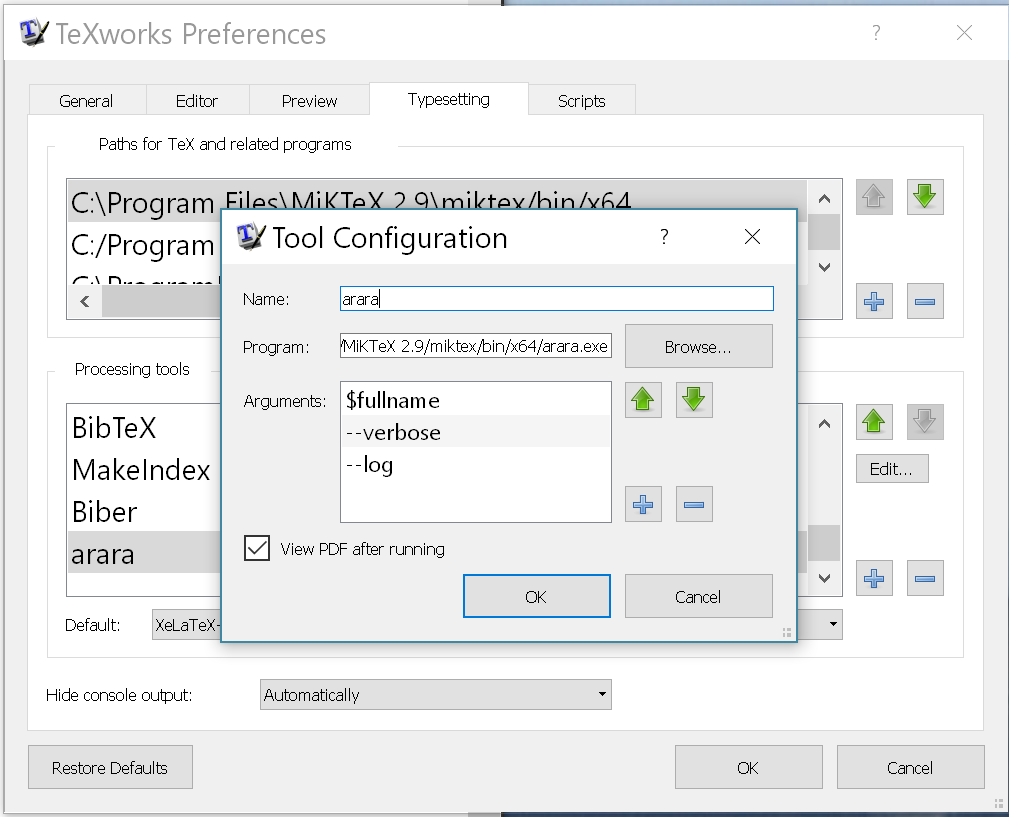
\includegraphics[scale=0.75]{../figs/arara.png}
\end{plScreen}
\vfill
\end{plSection}%{Typesetting}

%-----------------------------------------------------------------
%-----------------------------------------------------------------
\end{document}
%-----------------------------------------------------------------
